\pagebreak
\section{Метод решения}
Поиск работает над индексом из ЛР7 (\texttt{lab7/data/index.bin}: 1\,000\,000 документов Wikivoyage, Wikipedia, Travel Stack Exchange и Reddit, 3\,974\,421 терм). Компоненты:
\begin{itemize}
    \item \texttt{build/search} (C++) --- загрузка индекса, разбор и выполнение запросов, выдача. Чтение индекса --- общий с утилитой \texttt{lookup} ЛР7 заголовок \texttt{lab7/src/index\_reader.h}, слова запроса делятся на термы токенизатором ЛР3. Структуры данных собственные, без STL (STL --- только внутри токенизатора).
    \item \texttt{web/server.py} (Python, стандартная библиотека) --- веб-сервис, обвязка над \texttt{build/search}.
\end{itemize}
Индекс (1,6~ГиБ) читается в память целиком при запуске, около 0,9~с (файл в кэше ОС).

\subsection{Синтаксис запроса}
\begin{center}
\small
\begin{tabular}{|l|l|}
\hline
Операция & Запись \\
\hline
И & пробел, \texttt{\&\&}, \texttt{\&} (любое число амперсандов подряд) \\
\hline
ИЛИ & \texttt{\textbar\textbar}, \texttt{\textbar} (любое число палочек подряд) \\
\hline
НЕ & \texttt{!} перед словом или скобкой \\
\hline
Группировка & \texttt{( )} \\
\hline
\end{tabular}
\end{center}
Приоритет: НЕ выше И, И выше ИЛИ: \texttt{a b || c} --- это \texttt{(a \&\& b) || c}. Слово запроса делится на термы тем же токенизатором, что и документы, поэтому регистр не важен (\texttt{PARIS} = \texttt{paris}), а слово с дефисом или апострофом становится операцией И над частями (\texttt{Hewlett-Packard} $\to$ \texttt{hewlett \&\& packard}), --- так же оно разбито и в индексе.

\textbf{Разбор.} Лексер выделяет токены: \texttt{(}, \texttt{)}, \texttt{!}, серию \texttt{\&}, серию \texttt{|} и слово --- всё остальное до пробела или служебного символа. Парсер --- рекурсивный спуск по грамматике
\begin{center}
\small
\begin{tabular}{l}
\texttt{запрос \ \ := \{ или [ ")" ] \}} \\
\texttt{или \ \ \ \ \ := и \{ "||" и \}} \\
\texttt{и \ \ \ \ \ \ \ := \{ "\&\&" | унарное \}} \\
\texttt{унарное \ := "!" унарное | первичное} \\
\texttt{первичное := "(" или [ ")" ] | слово} \\
\end{tabular}
\end{center}
Подряд идущие операнды без оператора соединяются через И.

\textbf{Толерантность к вводу.} Запрос никогда не вызывает ошибку, а разбирается так, как его, скорее всего, имели в виду:
\begin{itemize}
    \item пробелы в любом количестве или без пробелов: \texttt{(red||yellow)car} = \texttt{(red || yellow) \&\& car};
    \item одиночные \texttt{\&} и \texttt{|} --- то же, что двойные;
    \item незакрытая скобка закрывается в конце запроса, лишняя закрывающая пропускается: \texttt{(lviv || kyiv} = \texttt{lviv || kyiv};
    \item оператор без операнда пропускается: \texttt{\&\& red ||} = \texttt{red}, \texttt{red !} = \texttt{red};
    \item двойное отрицание снимается: \texttt{!!red} = \texttt{red};
    \item пустые скобки и слова без букв и цифр (\texttt{---}, \texttt{,}) пропускаются; запрос, от которого ничего не осталось, даёт пустую выдачу.
\end{itemize}

Результат разбора --- дерево: лист --- терм, внутренние узлы --- И и ИЛИ с любым числом потомков (вложенные однотипные узлы сливаются: \texttt{(a b) c} = И(a, b, c)) и НЕ с одним потомком. Утилита печатает разобранный запрос в каноническом виде (строка \texttt{parsed:}), а веб-сервис показывает его пользователю --- видно, как понят запрос.

\subsection{Выполнение запроса}
Значение каждого узла --- упорядоченный по возрастанию массив docID.
\begin{itemize}
    \item \textbf{Терм} --- двоичный поиск в таблице термов индекса (около 20 сравнений строк), список документов копируется в массив. Нет терма --- пустой список.
    \item \textbf{И} --- вычисляются операнды без НЕ, сортируются по длине, затем пересекаются слиянием начиная с самого короткого: результат не длиннее самого короткого списка, а если он стал пустым, остальные списки не просматриваются. Операнды вида \texttt{!x} не вычисляются как дополнение, а вычитаются из результата: \texttt{a \&\& !b} = $a \setminus b$. Если у И только отрицания (\texttt{!a !b}), начальный результат --- все документы.
    \item \textbf{ИЛИ} --- объединение слиянием по очереди с каждым операндом.
    \item \textbf{НЕ} отдельно (\texttt{!a} целиком или внутри ИЛИ) --- дополнение до всех документов $0 \ldots N-1$.
\end{itemize}
Пересечение, объединение и разность двух списков --- один проход двумя указателями, $O(|a| + |b|)$. Выдача упорядочена по docID: ранжирования в булевом поиске нет.

\subsection{Утилита командной строки}
\texttt{search INDEX [-n LIMIT] [-o OFFSET] [-r REPEAT] < queries}: каждая строка входа --- запрос. На каждый запрос выводится блок:
\begin{verbatim}
query: <запрос как введён>
parsed: <разобранный запрос>
found: <число найденных документов>
time_us: <время разбора и выполнения, мкс>
<ранг> TAB <docID> TAB <заголовок> TAB <URL>   (LIMIT строк, по умолчанию 50)
<пустая строка>
\end{verbatim}
\texttt{-o} --- смещение (с какого результата выводить), \texttt{-n 0} --- все результаты, \texttt{-r} --- выполнить каждый запрос несколько раз и вывести среднее время (для замеров). Режим \texttt{-p} для веб-сервиса: строки вида \texttt{смещение TAB лимит TAB запрос}, после каждого блока вывод сбрасывается (\texttt{fflush}).

\subsection{Веб-сервис}
\texttt{python3 web/server.py --port 8080} --- HTTP-сервер из стандартной библиотеки Python. При запуске он один раз запускает \texttt{build/search} в режиме \texttt{-p} и дальше передаёт ему запросы через канал, так что индекс не загружается заново на каждый запрос (одновременные запросы ставятся в очередь блокировкой). Страницы:
\begin{itemize}
    \item \texttt{/} --- форма ввода запроса и подсказка по операторам;
    \item \texttt{/search?q=<запрос>\&p=<страница>} --- форма с введённым запросом, строка \enquote{как понят запрос, сколько найдено, какие показаны, время}, 50 результатов (заголовок --- ссылка на статью, под ним URL), ссылки \enquote{Предыдущие 50} и \enquote{Следующие 50}. Весь текст из запроса и индекса экранируется (\texttt{html.escape}).
\end{itemize}

\begin{center}
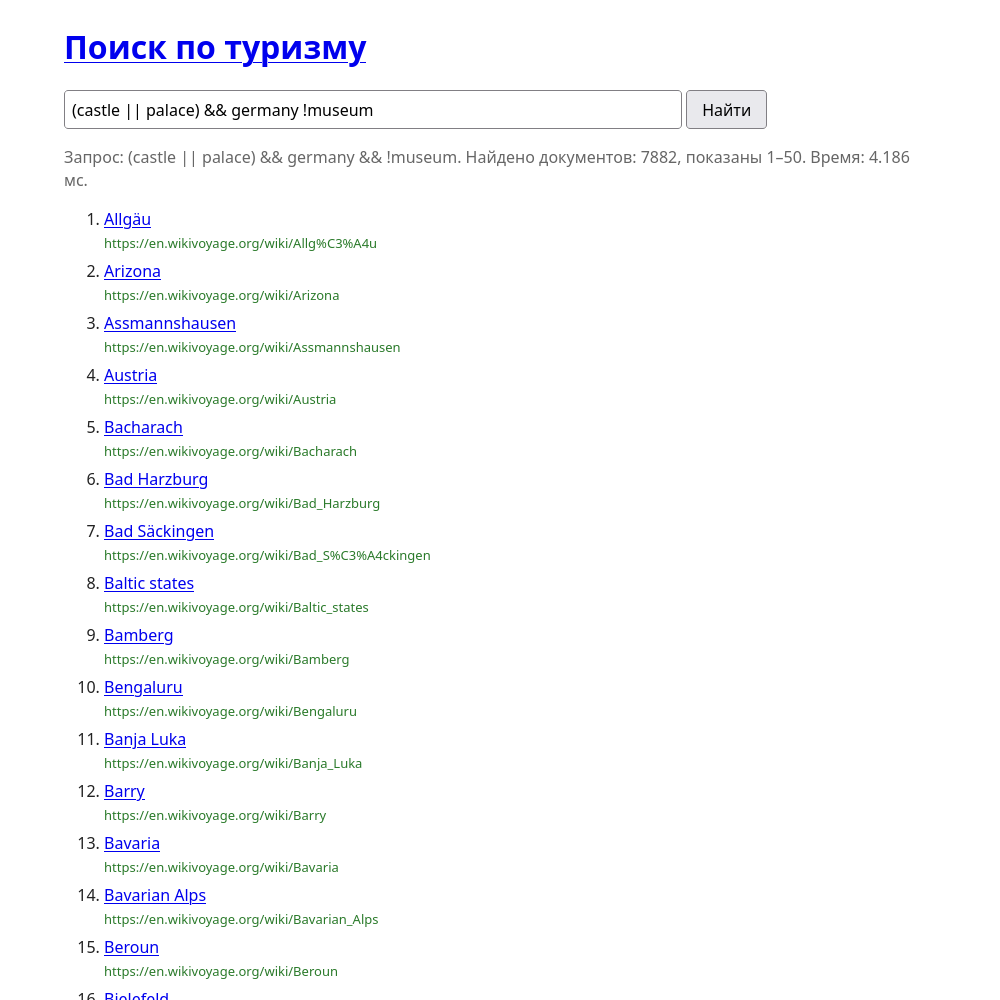
\includegraphics[width=0.8\textwidth]{img/search.png}

Страница выдачи веб-сервиса (снята \texttt{scripts/screenshot.py} через Firefox в режиме без окна)
\end{center}
